\documentclass[]{article}
\usepackage{lmodern}
\usepackage{amssymb,amsmath}
\usepackage{ifxetex,ifluatex}
\usepackage{fixltx2e} % provides \textsubscript
\ifnum 0\ifxetex 1\fi\ifluatex 1\fi=0 % if pdftex
  \usepackage[T1]{fontenc}
  \usepackage[utf8]{inputenc}
\else % if luatex or xelatex
  \ifxetex
    \usepackage{mathspec}
  \else
    \usepackage{fontspec}
  \fi
  \defaultfontfeatures{Ligatures=TeX,Scale=MatchLowercase}
\fi
% use upquote if available, for straight quotes in verbatim environments
\IfFileExists{upquote.sty}{\usepackage{upquote}}{}
% use microtype if available
\IfFileExists{microtype.sty}{%
\usepackage{microtype}
\UseMicrotypeSet[protrusion]{basicmath} % disable protrusion for tt fonts
}{}
\usepackage[margin=1in]{geometry}
\usepackage{hyperref}
\hypersetup{unicode=true,
            pdftitle={Data Analysis and Statistical Inference using R},
            pdfauthor={Student ID: 201081646},
            pdfborder={0 0 0},
            breaklinks=true}
\urlstyle{same}  % don't use monospace font for urls
\usepackage{longtable,booktabs}
\usepackage{graphicx,grffile}
\makeatletter
\def\maxwidth{\ifdim\Gin@nat@width>\linewidth\linewidth\else\Gin@nat@width\fi}
\def\maxheight{\ifdim\Gin@nat@height>\textheight\textheight\else\Gin@nat@height\fi}
\makeatother
% Scale images if necessary, so that they will not overflow the page
% margins by default, and it is still possible to overwrite the defaults
% using explicit options in \includegraphics[width, height, ...]{}
\setkeys{Gin}{width=\maxwidth,height=\maxheight,keepaspectratio}
\IfFileExists{parskip.sty}{%
\usepackage{parskip}
}{% else
\setlength{\parindent}{0pt}
\setlength{\parskip}{6pt plus 2pt minus 1pt}
}
\setlength{\emergencystretch}{3em}  % prevent overfull lines
\providecommand{\tightlist}{%
  \setlength{\itemsep}{0pt}\setlength{\parskip}{0pt}}
\setcounter{secnumdepth}{5}
% Redefines (sub)paragraphs to behave more like sections
\ifx\paragraph\undefined\else
\let\oldparagraph\paragraph
\renewcommand{\paragraph}[1]{\oldparagraph{#1}\mbox{}}
\fi
\ifx\subparagraph\undefined\else
\let\oldsubparagraph\subparagraph
\renewcommand{\subparagraph}[1]{\oldsubparagraph{#1}\mbox{}}
\fi

%%% Use protect on footnotes to avoid problems with footnotes in titles
\let\rmarkdownfootnote\footnote%
\def\footnote{\protect\rmarkdownfootnote}

%%% Change title format to be more compact
\usepackage{titling}

% Create subtitle command for use in maketitle
\newcommand{\subtitle}[1]{
  \posttitle{
    \begin{center}\large#1\end{center}
    }
}

\setlength{\droptitle}{-2em}

  \title{Data Analysis and Statistical Inference using R}
    \pretitle{\vspace{\droptitle}\centering\huge}
  \posttitle{\par}
    \author{Student ID: 201081646}
    \preauthor{\centering\large\emph}
  \postauthor{\par}
    \date{}
    \predate{}\postdate{}
  
\usepackage{floatrow}
\floatsetup[figure]{capposition=top}

\begin{document}
\maketitle

\section{Introduction}\label{introduction}

This report is the second assessment of the \textbf{MATH5741M
Statistical Theory and Methods} module. Its aim is to answer through
statistical analysis three questions regarding a road traffic accidents
dataset from 2005 collected by the UK Department for Transport.

All the analysis has been done using \textbf{R} (programming language)
and is code reproducible. To see the complete \textbf{R} coding process
and outputs visit
\url{https://github.com/eugenividal/Data_Analysis_and_Statistical_Inference_using_R}.

\section{Results}\label{results}

\subsection{Question 1}\label{question-1}

In this question, we are asked to draw a boxplot to compare the number
of vehicles involved in urban areas with the number involved in rural
areas.

For this, we first prepare the data removing ``Unallocated'' values from
the \texttt{Urban\_or\_Rural\ Area} variable. Then, we plot the graph.

\begin{figure}[H]

{\centering 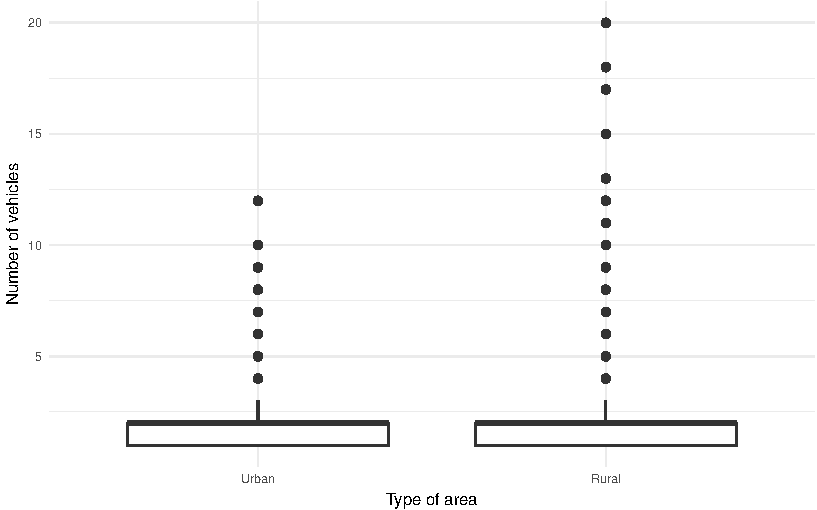
\includegraphics{README_files/figure-latex/fig-1} 

}

\caption{Number of vehicles involved in accidents grouped by type of area}\label{fig:fig}
\end{figure}

Apart from the fact that urban areas have less outliers than rural
areas, in the boxplot we cannot appreciate the differences between their
quantiles. Both boxes look identical and the median and upper quartile
seem to be coincident.

This is because the data is not symmetrical. As we can see in histogram
H1 (Figure 2), the data is very skewed to the right. To normalise it, we
transform the \texttt{Number\_of\_Vehicles} variable in three different
ways: taking the log10, log2 and using the square root (see histograms,
H2, H3 and H4 in Figure 2). In these new histograms, the distribution is
not entirely symmetric, but they have improved, particularly those that
take log10 and log2.

\begin{figure}[H]

{\centering 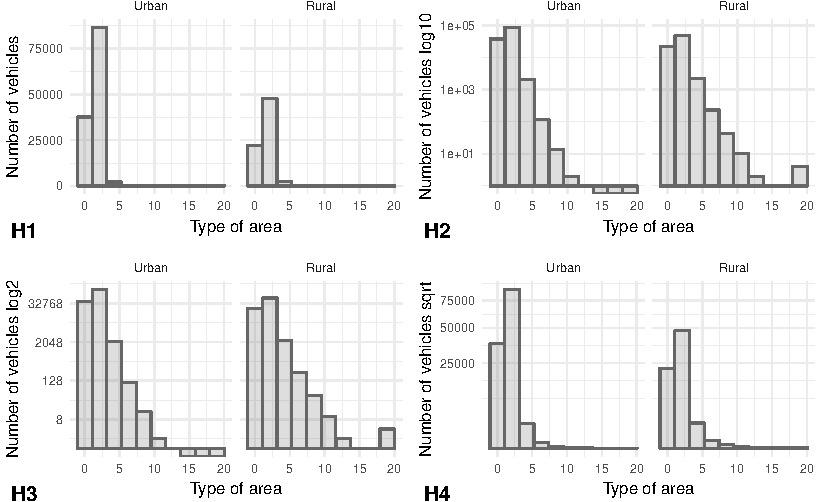
\includegraphics{README_files/figure-latex/fig2-1} 

}

\caption{Data histogram (H1) and transformed data histograms (H2, H3, H4)}\label{fig:fig2}
\end{figure}

We choose the log10 transformation and draw a second boxpot.

\begin{figure}[H]

{\centering 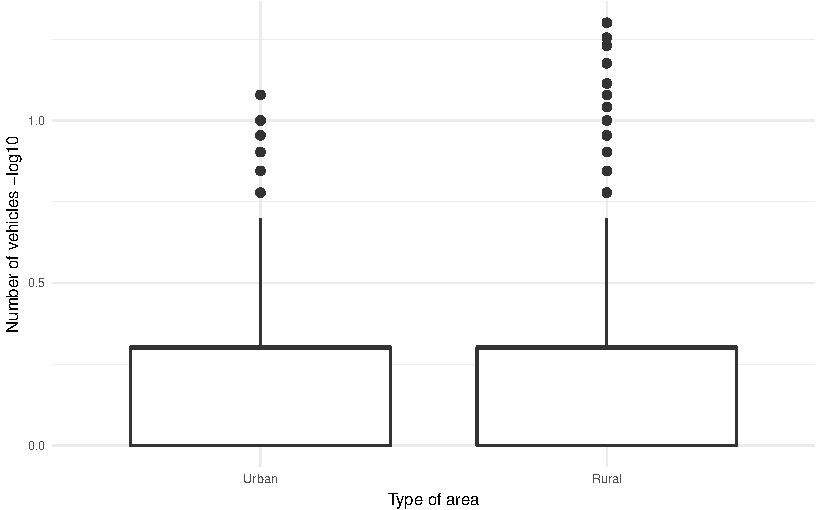
\includegraphics{README_files/figure-latex/fig3-1} 

}

\caption{Number of vehicles (log10) involved in accidents grouped by type of area}\label{fig:fig3}
\end{figure}

This time the appearance of the boxplot is better. However, the
interpretation can be even harder, and we cannot be 100\% sure whether
the average number of vehicles involved in accidents differs per type of
area.

To investigate this, we carry out a statistical test, which is the
second requirement of the question. The null hypothesis is that the mean
of vehicles involved in both types of areas is equal. The alternative
hypothesis is that they differ. Denoting the urban by subscript \emph{u}
and the rural areas by subscript \emph{r}, we have:

\[H_{0}: \mu_{u} = \mu_{r}\;\;\;vs.\;\;\;H_{1}: \mu_{u} \neq \mu_{r}\]
The summary statistics are:

\[n_{u}=126378\;\;\bar{x_{u}}=0.2305898\;\;s_{u}^{2}=0.02632197984\;\;n_{r}=72267\;\;\bar{x_{r}}=0.2389048\;\;s_{r}^{2}=0.03153835017\]

It seems reasonable to assume \(\sigma_{u}^{2}\) = \(\sigma_{r}^{2}\).
Consequently, we apply a \textbf{pooled variance} for our
estimates\footnote{We can assume equal variances when the ratio of
  max/min is less than 3 or less than 4 for small samples (Taylor 2017,
  69).}.

\[s_{p}^{2}=\frac{(n_{u}-1)s_{u}^{2}+(n_{r}-1)s_{r}^{2}}{n_{u}+n_{r}-2} = \frac{126377*0.02632197984+72266*0.03153835017}{126378+72267-2}=0.0282197\]

The test statistic is then:

\[\frac{\bar x_{u}-\bar x_{r}-0}{s_{p}\sqrt{\frac{1}{n_{u}}+\frac{1}{n_{r}}}}=\frac{0.2305898-0.2389048}{0.0007834463}=-10.61339\]

We compare this to the critical point of t-distribution with \(\nu\) =
198643 degrees of freedom\footnote{With this number of degrees of
  freedom we could have also apply z-statistic and the result would have
  been nearly the same.}, which is \(t_{198643}\)(0.005)=2.575854. Since
\textbar{}10.61339\textbar{} \textgreater{} 2.575854, we reject the null
hypothesis and conclude that the mean of vehicles involved in each type
of area is not equal (\(\mu_{u}\) \(\neq\) \(\mu_{r}\)).

\subsection{Question 2}\label{question-2}

In this question, we have to investigate whether the frequency of
accidents varies by day of the week using a suitable statistical
hypothesis test. \textbf{Chi-square test} can be used to test whether
observed data differ significantly from theoretical expectations (Lane
2018). So, this is the test we apply.

The null hypothesis is that the frequency of accidents is evenly
distributed per days of the week (i.e.~the probability of accidents
occurring per each day is 1/7). The alternative hypothesis is that their
frequency differs (i.e.~the probability of accidents occurring per each
day is not 1/7).

\[H_{0}: p=1/7\;\;\;vs.\;\;\;H_{1}:p\neq1/7\;\] \pagebreak

To carry out this test, first, we prepare the data, aggregating it by
\texttt{Day\_of\_Week}. Secondly, we create a table with the observed
values, the expected values and other necessary contributions for the
test per day of week.

\begin{longtable}[]{@{}rrrrr@{}}
\caption{Observed, expected and contributions to X\^{}2.
Mon-Sun}\tabularnewline
\toprule
week days & observed & expected & oi - ei & (oi -
ei)\^{}2/ei\tabularnewline
\midrule
\endfirsthead
\toprule
week days & observed & expected & oi - ei & (oi -
ei)\^{}2/ei\tabularnewline
\midrule
\endhead
Monday & 27812 & 28390.71 & 578.7143 & 11.79647\tabularnewline
Tuesday & 29219 & 28390.71 & -828.2857 & 24.16485\tabularnewline
Wednesday & 30373 & 28390.71 & -1982.2857 & 138.40640\tabularnewline
Thursday & 29738 & 28390.71 & -1347.2857 & 63.93565\tabularnewline
Friday & 32738 & 28390.71 & -4347.2857 & 665.67163\tabularnewline
Saturday & 26945 & 28390.71 & 1445.7143 & 73.61878\tabularnewline
Sunday & 21910 & 28390.71 & 6480.7143 & 1479.34487\tabularnewline
\bottomrule
\end{longtable}

The value of \(\chi ^2\) = 2456.93865. This can be compared to the
\(\chi ^2\) distribution with 7 - 1 = 6 degrees of freedom, giving a
p-value of 2.2e-16. This p-value represents the probability that we are
wrong in the assumption they are basically not equally distributed. So,
we reject the null hypothesis and affirm that the frequency of accidents
is not evenly distributed per days of the week (\(p\neq1/7\)).

Next, we are required to do the same test using only week-days
(excluding Saturday and Sunday).

This time, the null hypothesis is that the frequency of accidents is
equally distributed per week days (i.e.~the probability of accidents per
each week day is 1/5). The alternative hypothesis is that their
frequency differs (i.e.~the probability of accidents per each week day
is not 1/5).

\[H_{0}: p=1/5\;\;\;vs.\;\;\;H_{1}:p\neq1/5\;\]

First, we prepare the data, aggregating it by \texttt{Day\_of\_Week} and
removing Saturday and Sundays. Then, we create a new table with the
summaries from Monday to Friday.

\begin{longtable}[]{@{}rrrrr@{}}
\caption{Observed, expected and contributions to X\^{}2.
Mon-Fri}\tabularnewline
\toprule
week days & observed & expected & oi - ei & (oi -
ei)\^{}2/ei\tabularnewline
\midrule
\endfirsthead
\toprule
week days & observed & expected & oi - ei & (oi -
ei)\^{}2/ei\tabularnewline
\midrule
\endhead
Monday & 27812 & 29976 & 2164 & 156.221510\tabularnewline
Tuesday & 29219 & 29976 & 757 & 19.116927\tabularnewline
Wednesday & 30373 & 29976 & -397 & 5.257840\tabularnewline
Thursday & 29738 & 29976 & 238 & 1.889645\tabularnewline
Friday & 32738 & 29976 & -2762 & 254.491727\tabularnewline
\bottomrule
\end{longtable}

The value of \(\chi ^2\) = 436.9776. This is compared to the \(\chi ^2\)
distribution with 5-1=4 degree of freedom, giving a p-value again of
2.2e-16. So, again we reject the null hypothesis and state that the
frequency of accidents in week days is not equally distributed
(\(p\neq1/5\)).

\subsection{Question 3}\label{question-3}

Finally, we are asked to compute a 95\% confidence interval for the
expected (mean) number of accidents which occur on a Monday.

To prepare the data, we filter the accidents occurred on Mondays and
group them by date.

In total we get 52 observations (\(n\) = 52). The sample mean and
standard deviation are: \(\bar{x}\)= 534.8462 and \(s\)= 92.98627
respectively. Since we desire a 95\% interval, our \(\alpha\)= 0.05. We
then find that \(t_{51}(0.025)\)= 2.007584.

Substituting all these quantities into the form of the confidence
interval, we have the 95\% confidence interval for the expected number
of accidents on a Monday.

\[\left ( \bar{x} -t_{n-1}(\alpha /2)\frac{s}{\sqrt{n}}, \bar{x} +t_{n-1}(\alpha /2)\frac{s}{\sqrt{n}}\right) = (534.8462-25.88754,\; 534.8462+25.88754) = 508.9586, 560.7337\]

Computing this interval, we state the assumption that the data are
normally distributed. An informal approach to check that this assumption
is reasonable, is to compare a histogram (or another kind of graph) of
the sample data to a normal probability curve, as we did in question 1.

\begin{figure}[H]

{\centering 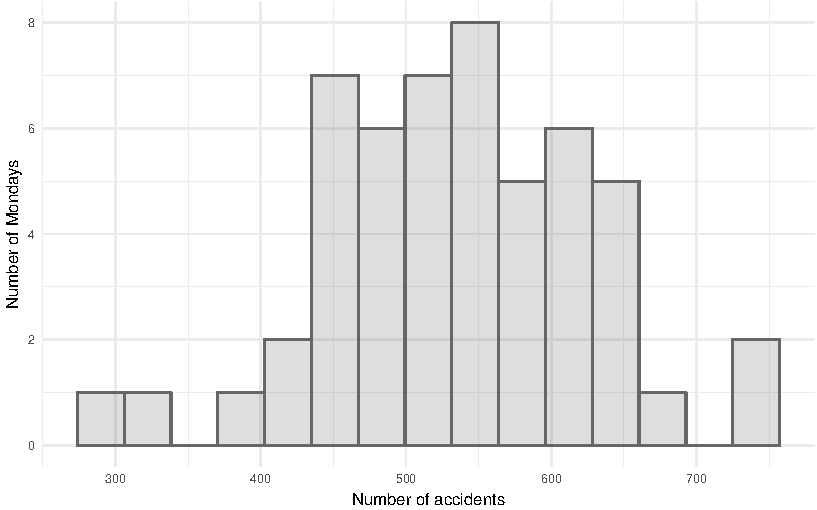
\includegraphics{README_files/figure-latex/fig5-1} 

}

\caption{Histogram number of accidents which occur on a Monday}\label{fig:fig5}
\end{figure}

The histogram does not show perfect symmetry, but its shape is close to
normal distribution.

However, to be more certain, various formal hypothesis tests to check
normality can be used. The one that we will use here is the
\textbf{Shapiro-Wilk test}, which takes account of the expected values,
but also the correlations between the order statistics (Taylor 2017,
85).

These are the hypothesis:

\[H_{0}: data\;come\;from\;a\;normal\;distribution\;\;\;vs.\;\;\;H_{1}:data\;do\;not\;come\;from\;a\;normal\;distribution\]

To perform the test we use the command \texttt{shapiro.test(x)} in
\textbf{R}.

The results are W = 0.98537 and p-value = 0.7681.

The p-values gives evidence against the null hypothesis. Since the
p-value = 0.7681 is large (i.e.~greater than 0.05), we accept that the
data come from a normally distributed population.

\section*{References}\label{references}
\addcontentsline{toc}{section}{References}

\hypertarget{refs}{}
\hypertarget{ref-lane_online_2018}{}
Lane, David M. 2018. ``Online Statistics Education: An Interactive
Multimedia Course of Study.'' \url{http://onlinestatbook.com/}.

\hypertarget{ref-taylor_math5741m:_2017}{}
Taylor, Charles. 2017. ``MATH5741M: Statistical Theory and Methods.''
School of Mathematics - University of Leeds.


\end{document}
